\documentclass[
12pt,				% Font size
openright,			% 
oneside,			% Enables one side print
a4paper,			% Paper size 
english,			% Main language hyphenation
french,				% Second language hyphenation
spanish,			% Third language hyphenation
brazil,				% Document main language
twocolumn			% Enables two column parts
]{abntex2}

% Packages used
% Basic packages 

% Enables the use of acronyms
\usepackage[
	printonlyused, 
	footnote, 
	withpage
]{acronym}

% Enables custom datetimes
\usepackage[useregional]{datetime2}

% Enables text replacing
\usepackage{xstring}

% Enable long tables
\usepackage{longtable}

% Enable cvs data load
\usepackage{csvsimple, booktabs}

% Allow more floats whatever is this
\usepackage{morefloats}

% Use latim special characters
\usepackage[utf8]{inputenc}

\usepackage[T1]{fontenc}

% Use colors
\usepackage{color}

% Enables landscape pages
\usepackage{lscape}

% Enables graphics
\usepackage{graphicx}

% Better text justification
% DO NOT ENABLE THIS! OTHERWISE
% IT WILL MESSUP ABNTEX2
%\usepackage{microtype}

% Indent the section first paragraph.
\usepackage{indentfirst}

% Tables colors!!
\usepackage[table]{xcolor}

% Enables code listing
\usepackage{listings}

% Enables multicolumn text
\usepackage{multicol}

% Enables math
\usepackage{amsthm}
\usepackage{amsmath, mathtools}
\usepackage{amssymb}
\usepackage{cancel}

% Adds some symbols (like slash on a non mathematical context)
\usepackage{textcomp}

% Enables the use of subfigures
\usepackage{subfig}

% Float barriers, prevents figures floats accross
% an determined \FloatBarrier
\usepackage[section]{placeins}

% Eanbles the use of landscape pages
\usepackage{lscape}
\usepackage{pdflscape}

% Quote packages
% ABNT standard
\usepackage[
	alf,
	abnt-etal-text=it,
	abnt-etal-list=0,
	abnt-missing-year=sd
]{abntex2cite}

% Bibliography 
\usepackage[
	brazilian,
	hyperpageref
]{backref}

% Drawing and plot packages
\usepackage{relsize}
\usepackage{tikz}
\usetikzlibrary{calc}
\usetikzlibrary{datavisualization}
\usetikzlibrary{positioning}
\usetikzlibrary{mindmap}
\usetikzlibrary{snakes}
\usetikzlibrary{shapes}
\usetikzlibrary{decorations.pathreplacing}
\usetikzlibrary{spy}
\usetikzlibrary{backgrounds}
\usetikzlibrary{patterns}
\usetikzlibrary{fit}

\usepackage{pgfplots}
\usepackage{pgfplotstable}
\pgfplotsset{compat=newest}
\usepgfplotslibrary{units}

% Packages configuration

% Long tables pre and post spacing
\setlength{\LTpre}{0pt}
\setlength{\LTpost}{-30pt}

% Backref confis
\renewcommand{\backrefpagesname}{Citado na(s) página(s):~}
\renewcommand{\backref}{}

% Quote text
\renewcommand*{\backrefalt}[4]{
	\ifcase #1
	
	\or
	Citado na página #2.
	\else
	Citado #1 vezes nas páginas #2.
	\fi}

% Solves some problems that appears when some text is copied and pasted with some unicode chars
\DeclareUnicodeCharacter{200B}{{\hskip 0pt}}

% Document and author informations (you can edit it)
% Put here the day, month and the year of your document
\renewcommand{\day}{06}
\renewcommand{\month}{Agosto}
\renewcommand{\year}{2022}

% Do not touch here!!!
\renewcommand{\today}{\day \space de \month \space de \year}
\newcommand{\enUSkeyWords}{
	{paraconsistent analysis}, 
	{imagined speech}, 
	{wavelet}, {wavelet-packet}, {SNN}, {spiking neural networks}, {EEG}
}

\newcommand{\ptBRkeyWords}{
	{análise paraconsistente}, 
	{imagined speech}, 
	{wavelet}, {wavelet-packet}, {SNN}, {redes neurais de pulso}, {EEG}
}
\titulo{Caracterização de \textit{voice spoofing} para fins de verificação de locutores com base na Transformada \textit{Wavelet} e na análise paraconsistente de características}
\autor{André Furlan}
\local{São José do Rio Preto}
\data{\year}
\orientador{Prof. Dr. Rodrigo Capobianco Guido}
\tipotrabalho{Dissertação para obtenção do título de Mestre em Ciência da Computação}
\preambulo{Dissertação apresentada como parte dos requisitos para obtenção do título de Mestre em Ciência da Computação, junto ao Programa de Pós-Graduação em Ciência da Computação, do Instituto de Biociências, Letras e Ciências Exatas da Universidade Estadual Paulista `Júlio de Mesquita Filho", Campus de São José do Rio Preto.}

% Code listing settings
% Translate Listing -> Algoritmo
\renewcommand{\lstlistingname}{Algoritmo}
% Translate List of Listings -> Lista de Algoritmos
\renewcommand{\lstlistlistingname}{Lista de \lstlistingname s}

% The code style
\definecolor{codegreen}{rgb}{0,0.6,0}
\definecolor{codegray}{rgb}{0.5,0.5,0.5}
\definecolor{codepurple}{rgb}{0.58,0,0.82}
\definecolor{backcolour}{rgb}{0.95,0.95,0.92}

% Defines code listing style
\lstdefinestyle{mystyle}{
	backgroundcolor=\color{backcolour},   
	commentstyle=\color{codegreen},
	keywordstyle=\color{magenta},
	numberstyle=\tiny\color{codegray},
	stringstyle=\color{codepurple},
	basicstyle=\ttfamily\footnotesize,
	breakatwhitespace=false,         
	breaklines=true,                 
	captionpos=b,                    
	keepspaces=true,                 
	numbers=left,                    
	numbersep=5pt,                  
	showspaces=false,                
	showstringspaces=false,
	showtabs=false,                  
	tabsize=2
}

\lstset{style=mystyle}

% Forces a new page
\newcommand{\forceNewPage}{
	\FloatBarrier
	\clearpage
	\newpage
}

% Toggle off clearpage
\newcommand{\disableClearpage}{
	\let\oldclearpage\clearpage
	\let\clearpage\relax
}

% Toggle on clearpage
\newcommand{\enableClearpage}{
	\let\clearpage\oldclearpage
}

% Redefine cover macro
\renewcommand{\imprimircapa}{%
	\begin{capa}%
		\center
		\centering 
\includegraphics[angle=-90]{unesp.pdf}
		\vspace{3cm}
		\par {\ABNTEXchapterfont\Large\imprimirautor}
		\vfill
		\begin{center}
			\ABNTEXchapterfont\LARGE\huge\imprimirtitulo
		\end{center}
		\vfill
		\ABNTEXchapterfont \large\imprimirlocal\\
		\large\imprimirdata
		\vspace*{1cm}
	\end{capa}
}

% Redefine face macro
\renewcommand{\folhaderostocontent}{
	\begin{center}
		
		%\vspace*{1cm}
		\ABNTEXchapterfont\large\imprimirautor
		
		\vspace*{\fill}
		\vspace*{\fill}
		\begin{center}
			\ABNTEXchapterfont\LARGE\imprimirtitulo
		\end{center}
		\vspace*{\fill}
		
		\hspace{.45\textwidth}
		\begin{minipage}{.5\textwidth}
			\SingleSpacing
			\imprimirpreambulo
		\end{minipage}%
		\vspace*{\fill}
		
		\imprimirinstituicao\vspace*{\fill}
		
		\large\imprimirorientadorRotulo~\imprimirorientador
		
		\vspace*{\fill}
		
		\large\imprimirlocal
		\par
		\large\imprimirdata
		\vspace*{1cm}
		
	\end{center}
}

% Pdf informations
\makeatletter
\hypersetup{
	pdftitle={\@title}, 
	pdfauthor={\@author},
	pdfsubject={\imprimirpreambulo},
	pdfcreator={LaTeX with abnTeX2},
	pdfkeywords={\ptBRkeyWords, \enUSkeyWords}, 
	colorlinks=true,       		% false: boxed links; true: colored links
	linkcolor=black,          	% color of internal links
	citecolor=black,        		% color of links to bibliography
	filecolor=black,      	% color of file links
	urlcolor=black,
	bookmarksdepth=4
}
\makeatother

% Put orfan images on the top of page. 
% See https://github.com/abntex/abntex2/issues/170
\makeatletter
\setlength{\@fptop}{5pt}
\makeatother

% Enables the creation of frame en frame lists.
% See https://github.com/abntex/abntex2/issues/176
\newcommand{\quadroname}{Quadro}
\newcommand{\listofquadrosname}{Lista de quadros}
\newfloat[chapter]{quadro}{loq}{\quadroname}
\newlistof{listofquadros}{loq}{\listofquadrosname}
\newlistentry{quadro}{loq}{0}

% ABNT settings
\setfloatadjustment{quadro}{\centering}
\counterwithout{quadro}{chapter}
\renewcommand{\cftquadroname}{\quadroname\space} 
\renewcommand*{\cftquadroaftersnum}{\hfill--\hfill}

% See https://github.com/abntex/abntex2/issues/176
\setfloatlocations{quadro}{hbtp} 

% Paragraph size
\setlength{\parindent}{1.3cm}

% Beetween paragraph spacing:
\setlength{\parskip}{0.2cm}  % tente também \onelineskip

% Document language
\selectlanguage{brazil}

% Builds the index
\makeindex

% Remove useless extra spaces
\frenchspacing 

% By default this is a one column document, use	\twocolumn to enable two columns
\onecolumn
% For some reason i couldn't put this package in the
% chapters/data/packages.tex file. If i do, tex raises
% a "there is no begin(document)" error
\usepackage{float}

\title{Autenticação Biométrica de Locutores Drasticamente Disfônicos Aprimorada pela \textit{Imagined Speech}}

\institute{Universidade Estadual Paulista Júlio de Mesquita Filho}

\author{André Furlan - ensismoebius@gmail.com}

\logo{
\includegraphics[height=1cm]{unesp.png}}
\date{\the\year}

\begin{document}
	
	\frame{\titlepage}
	
	\section{Introdução}
		\begin{frame}
	\frametitle{Introdução}
	
	\only<1>{
		\framesubtitle{Motivações e contextualização}
		\par A autenticação biométrica tem sido amplamente adotada por fornecer individualização baseada em traços únicos dos indivíduos. No entanto, características físicas que diferem das esperadas pelo sistema podem dificultar ou impedir o acesso de certas pessoas, especialmente aquelas pertencentes a grupos étnicos minorizados ou com deficiências. No caso da autenticação por voz, a exigência de uma palavra-chave ou outro tipo de fonação pode criar barreiras adicionais. Para mitigar esse problema, este trabalho propõe um sistema de autenticação biométrica aprimorado pela fala imaginada.
	}
	\only<2>{		
		\framesubtitle{Objetivos}
		\begin{itemize}
			\item Criar um sistema de autenticação por voz aprimorado pela fala imaginada.
			
			\item Comparar o desempenho das estratégias de extração de características automatizadas com o uso de autoencoders com as que usam \textit{Wavelet-Packet} de tempo discreto e engenharia paraconsistente de características.
			
			\item Criar uma base com dados de autenticação voz, fala imaginada e ambos os sinais simultâneos fornecendo a comunidade cientifica mais uma fonte de dados.
		\end{itemize}
	}
\end{frame}

	\section{Estrutura da apresentação}
		\begin{frame}
	\frametitle{Estrutura da apresentação}
	\begin{itemize}
		\item Revisão de conceitos utilizados.
		\item Estado-da-arte em Playback Speech Detection.
		\item Contextualização.
		\item Abordagem proposta.
		\item Testes e resultados.
		\item Conclusões e Trabalhos Futuros.
	\end{itemize}
\end{frame}

	\section{Revisão de conceitos utilizados}
		\begin{frame}
	\frametitle{Introdução}
	\par Para desenvolver o trabalho, é necessário definir os conceitos de \textit{downsampling}, filtros digitais \textit{wavelets} e energia, que serão usados para a extração de características dos sinais. No processamento dos sinais de voz, serão revisadas as frequências fundamentais da voz, além das escalas BARK e MEL. Também será revisada a engenharia paraconsistente de características, método utilizado para verificar a qualidade das características extraídas. Em seguida, serão estudadas as bases das interfaces Humano-Máquina para eletroencefalograma, que coletarão dados das regiões do cérebro. Concluída essa etapa, serão revisadas as redes neurais de pulso, autoencoders e redes neurais residuais.
\end{frame}
		\begin{frame}
	\frametitle{Sinais Digitais e Sub-amostragem (Downsampling)}
	\begin{figure}
		\centering
		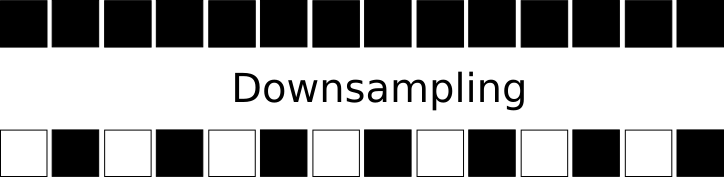
\includegraphics[width=0.5\linewidth]{../monography/images/downsampling}
		\caption{Sub-amostragem}
		\label{fig:downsampling}
	\end{figure}
	\par Ocorre após a conversão de domínio dos sinais com base em filtros digitais do tipo \textit{wavelet}.
\end{frame}
		\begin{frame}
	\frametitle{Caracterização dos processos de produção da voz humana}
	\only<1>{
		\framesubtitle{Áreas de estudo}
		\begin{itemize}
			\item fisiológica ou “fonética articulatória”.
			\item acústica ou “fonética acústica”.
			\item perceptual.
		\end{itemize}
		\par Neste trabalho, o foco será apenas na questão acústica, pois não serão analisados aspectos da fisiologia relacionada à voz, mas sim os sinais sonoros propriamente ditos.
	}
	\only<2>{
		\framesubtitle{Vozeada versus não-vozeada}
		\begin{itemize}
			\item vozeada: Pregas vocais.
			\item não vozeada: Sem pregas vocais.
		\end{itemize}
	}
	\only<3>{
		\framesubtitle{Frequência fundamental da voz}
		\begin{itemize}
			\item conhecida como $F_0$ representa o tom ou \textit{pitch} da voz \cite{kremer2014eficiencia}.
			\item reflete a excitação pulmonar moldada pelas pregas vocais.
			\item componente periódico resultante da vibração das pregas vocais.
			\item geralmente são apresentadas em Hz \cite{freitas2013avaliaccao}
		\end{itemize}
		
		\vspace{3em}
		
		\par A alteração desta frequência (jitter) e/ou intensidade (shimmer) do \textit{pitch} durante a fala é definida como entonação,  porém, também pode indicar algum distúrbio ou doença relacionada ao trato vocal \cite{WERTZNER2005}.
	}
	\only<4>{
		\framesubtitle{Formantes}
		\par Se referem as modificações feitas em $F_0$ pelas estruturas do sistema fonador \cite{valencca2014analise}:
		\begin{itemize}
			\item $F_1 \rightarrow$ amplificação  sonora  na  cavidade  oral  posterior,  posição  da  língua  no  plano  vertical.
			\item $F_2 \rightarrow$ cavidade  oral  anterior,  posição  da  língua  no  plano  horizontal.
			\item $F_3 \rightarrow$ cavidades  à  frente  e  atrás  do  ápice  da  língua.
			\item $F_4 \rightarrow$ formato da laringe e da  faringe.
		\end{itemize}
	}
\end{frame}
		\begin{frame}
	\frametitle{Bandas críticas de energia}
		\only<1>{
			\framesubtitle{Definições}
			\par Definem os intervalos em que serão calculadas as energias.\newline
			\begin{columns}
				\column{0.5\textwidth}
					\par A energia de um sinal digital $s[\cdot]$ com $M$ amostras é definida como
					\begin{equation}
						E = \sum\limits_{i=0}^{M-1}(s_i)^2 \qquad.   
					\end{equation}
				\column{0.5\textwidth}
					\begin{itemize}
						\item \textbf{BARK:} 20, 100, 200, 300, 400, 510, 630, 770, 920, 1080, 1270, 1480, 1720, 2000, 2320, 2700, 3150, 3700, 4400, 5300, 6400, 7700, 9500, 12000, 15500 (bandas de audição humana) \cite{doi:10.1121-1.1908630}.
						\item \textbf{MEL:} 20, 160, 394, 670, 1000, 1420, 1900, 2450, 3120, 4000, 5100, 6600, 9000, 14000 (bandas de audição adaptada para voz) \cite{beranek1949acoustic}.
					\end{itemize}
			\end{columns}
		}
		\only<2>{
			\framesubtitle{Cálculo de vetores de características com BARK}
			\begin{figure}
				\centering
				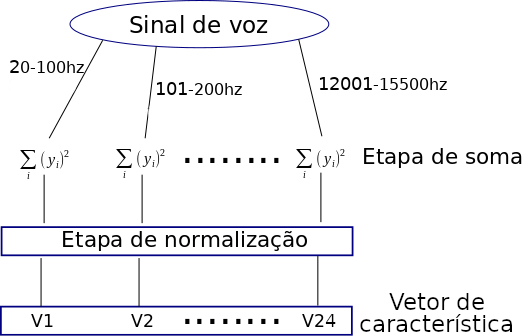
\includegraphics[width=0.7\linewidth]{../monography/images/barkFeatureVect}
			\end{figure}
		}
		\only<3>{
			\framesubtitle{Cálculo de vetores de características com MEL}
			\begin{figure}
				\centering
				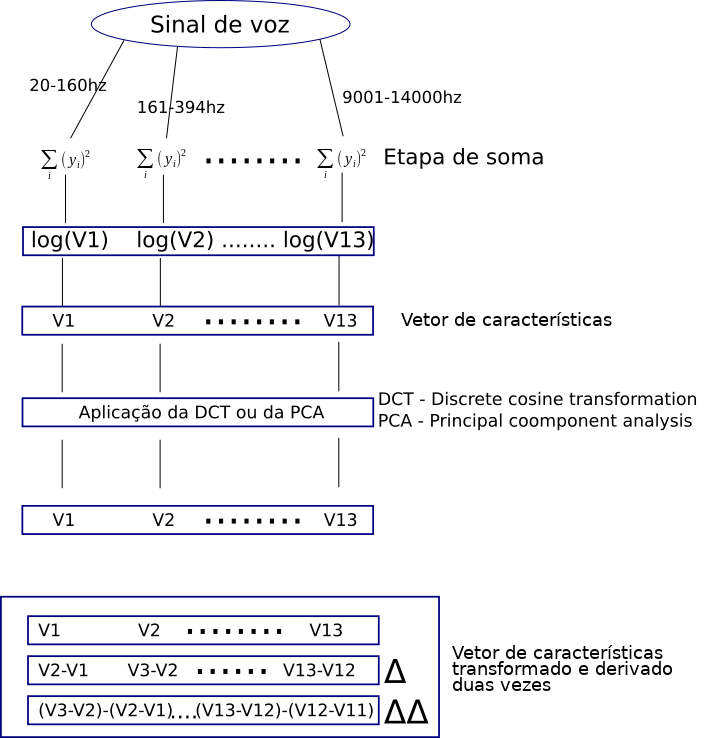
\includegraphics[width=0.5\linewidth]{../monography/images/melFeatureVect}
			\end{figure}
		}
\end{frame}
		\begin{frame}
	\frametitle{Filtros digitais \textit{wavelet}}
	\only<1>{
		\framesubtitle{Propriedades}
		\begin{itemize}
			\item suporte compacto.
			\item análise multirresolução.
			\item wavelet regular e wavelet packet.
			\item variadas funções-filtro não-periódicas.
			\item análise detalhada em altas e baixas frequências.
		\end{itemize}
	}
	\only<2>{
		\framesubtitle{Restrição de escopo}
		\begin{itemize}
			\item wavelet packet
			\item domínio discreto.
			\item apenas transformadas diretas.
			\item não haverá reconstrução do sinal.
			\item construção dos vetores de características.
		\end{itemize}
	}

	\only<3>{
		\framesubtitle{Resposta em frequência e linearidade}
		\begin{table}[h]
	\centering
	\caption{Algumas das \textit{wavelets} mais usadas e suas propriedades}
	\begin{tabular}{|c|p{75mm}|c|}
			\hline 
			\textbf{Wavelet} & \textbf{Resposta em frequência} & \textbf{Resposta em fase} \\ 
			\hline 
			Haar & Pobre &  Linear \\ 
			\hline 
			Daubechies & mais próxima da ideal à medida que o \newline  suporte aumenta; \textit{maximally-flat}  &  Não linear \\ 
			\hline 
			Symmlets & mais próxima da ideal à medida que o \newline  suporte aumenta; não \textit{maximally-flat}  & Quase linear \\ 
			\hline 
			Coiflets & mais próxima da ideal à medida que o \newline  suporte aumenta; não \textit{maximally-flat}  & Quase linear \\ 
			\hline 
	\end{tabular} 
	\label{tab:waveletsProperties}
	\\Fonte: Elaborado pelo autor, 2022.
\end{table}

	}

	\only<4>{
		\framesubtitle{Algoritmo de Malat}
		\begin{itemize}
			\item \textit{Wavelet} Haar: $h[\cdot] = [\frac{1}{\sqrt{2}}, \frac{1}{\sqrt{2}}]$.
			\item Par ortogonal: $g[\cdot] = [\frac{1}{\sqrt{2}}, \frac{-1}{\sqrt{2}}]$.
			\item sinal: $s[\cdot] = [1,2,3,4]$.
		\end{itemize}
		
		\begin{equation*}
			\begin{pmatrix}
			\frac{1}{\sqrt{2}}, \frac{1}{\sqrt{2}}, 0, 0\\
			\frac{1}{\sqrt{2}}, \frac{-1}{\sqrt{2}}, 0, 0\\
			0, 0, \frac{1}{\sqrt{2}}, \frac{1}{\sqrt{2}}\\
			0, 0, \frac{1}{\sqrt{2}}, \frac{1}{\sqrt{2}}\\
			\end{pmatrix} 
			\cdot
			\begin{pmatrix}
			1\\
			2\\
			3\\
			4\\
			\end{pmatrix} 
			=
			\begin{pmatrix}
			\frac{3}{\sqrt{2}}\\
			\frac{-1}{\sqrt{2}}\\
			\frac{7}{\sqrt{2}}\\
			\frac{-1}{\sqrt{2}}\\
			\end{pmatrix}
			\Rightarrow \Big[
			\frac{3}{\sqrt{2}},
			\frac{7}{\sqrt{2}},
			\frac{-1}{\sqrt{2}},
			\frac{-1}{\sqrt{2}}
			\Big]\qquad.
		\end{equation*}
	}

	\only<5>{
		\framesubtitle{Exemplo de \textit{wavelet} regular e \textit{packet}}
		\begin{figure}
			\centering
			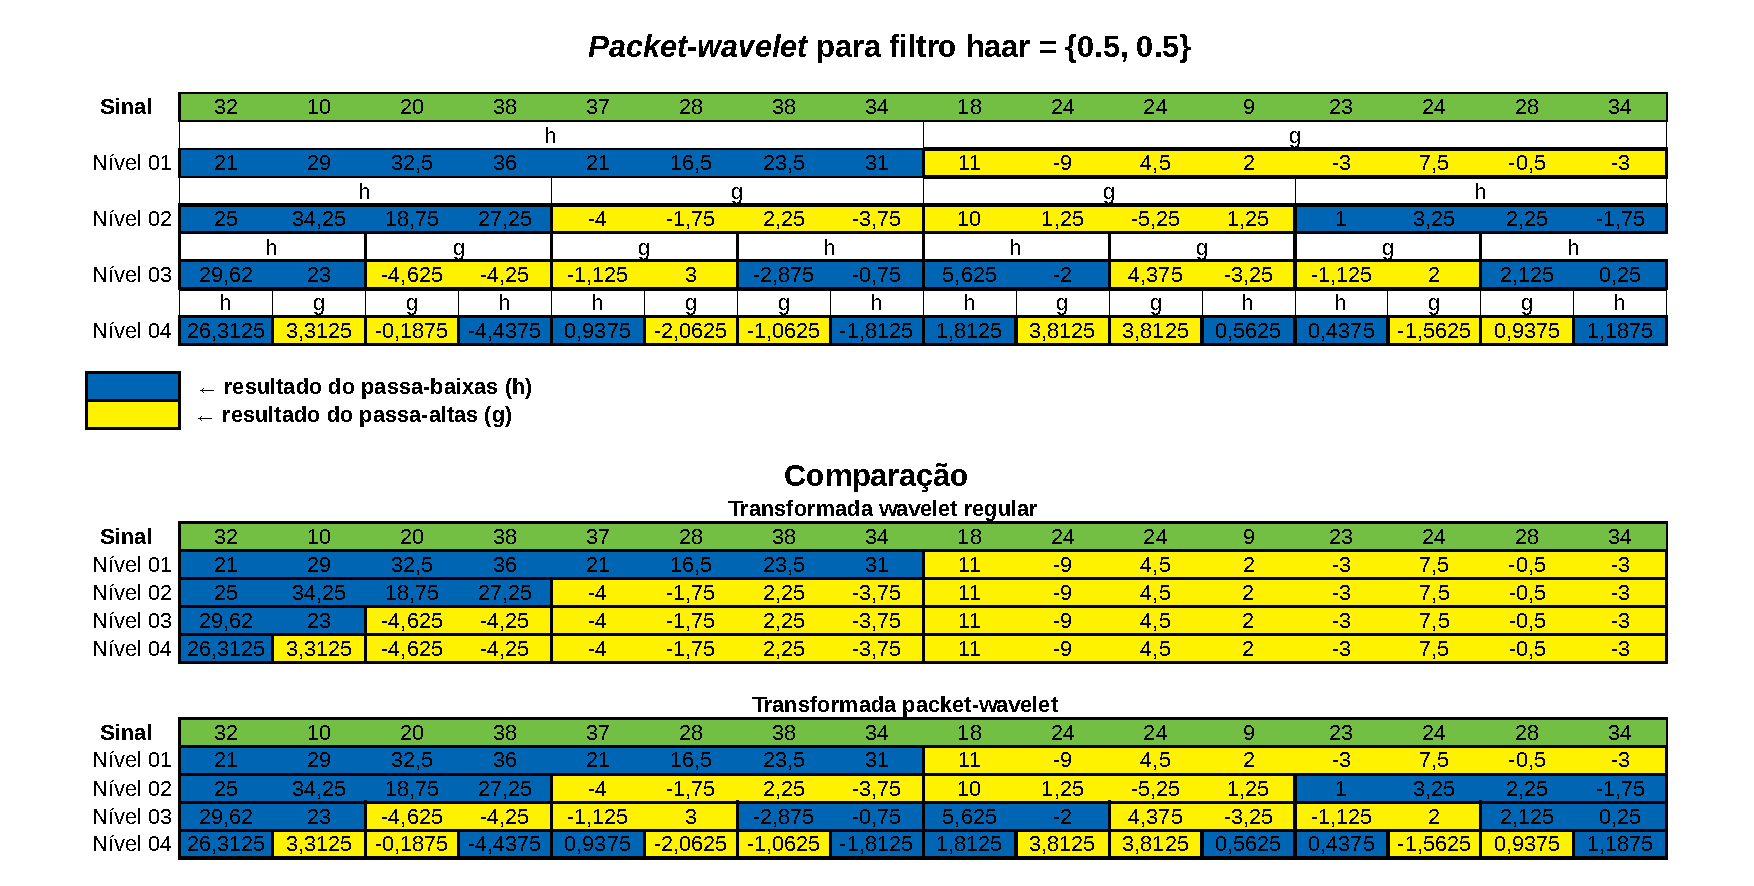
\includegraphics[width=\linewidth]{../monography/images/haarWaveletExamples}
		\end{figure}
	}

	\only<6>{
		\framesubtitle{Porquê e \textit{wavelet packet}?}
		\begin{itemize}
			\item decompõe a aproximação e os detalhes
			\item proporciona um nível de decomposição maior
		\end{itemize}
	}
\end{frame}








		\begin{frame}
	\frametitle{Engenharia paraconsistente de características}
	\only<1>{
		\framesubtitle{Cálculo de $\alpha$}
		\begin{columns}
			\column{.5\textwidth}
			\begin{textblock*}{0cm}(.4cm,1.5cm)
				\centering
				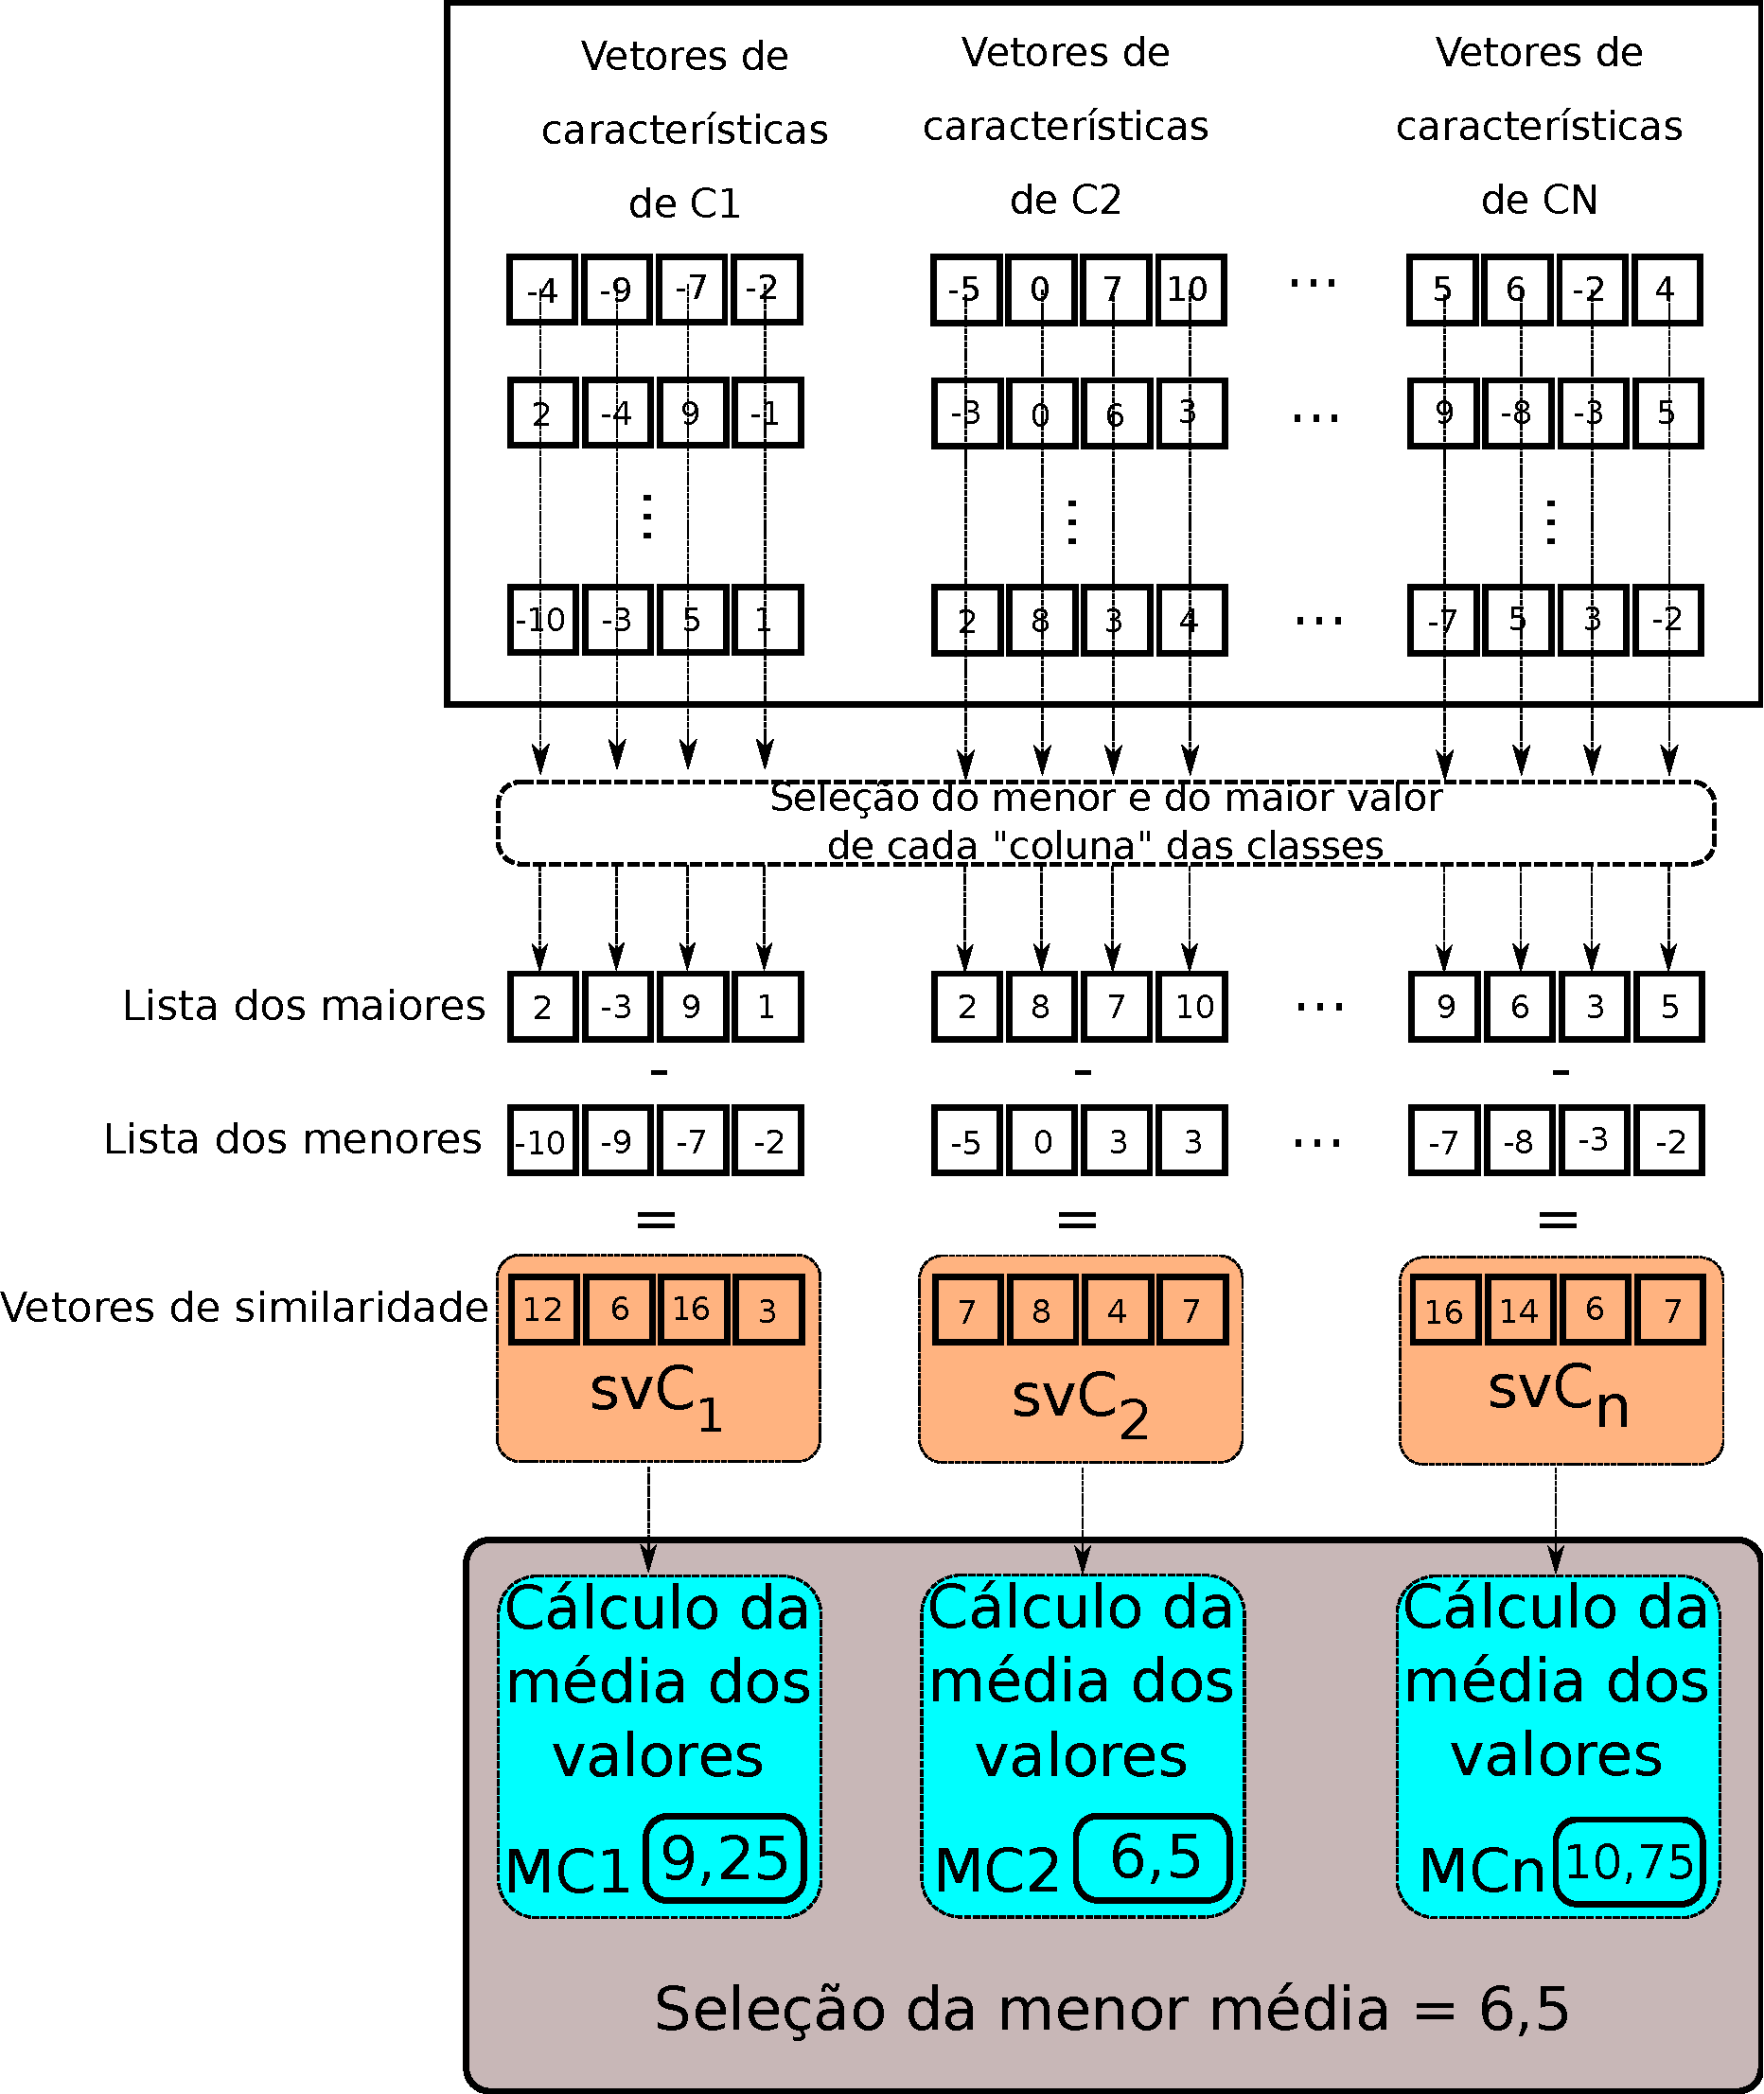
\includegraphics[height=0.82\textheight]{../monography/images/calculoAlpha.pdf}
			\end{textblock*}
			\column{.5\textwidth}
			\par Menor similaridade intraclasse, $\alpha$
		\end{columns}
	}
	\only<2>{
		\framesubtitle{Cálculo de $\beta$}
		\begin{columns}
			\column{.5\textwidth}
			\begin{textblock*}{0cm}(.4cm,1.5cm)
				\centering
				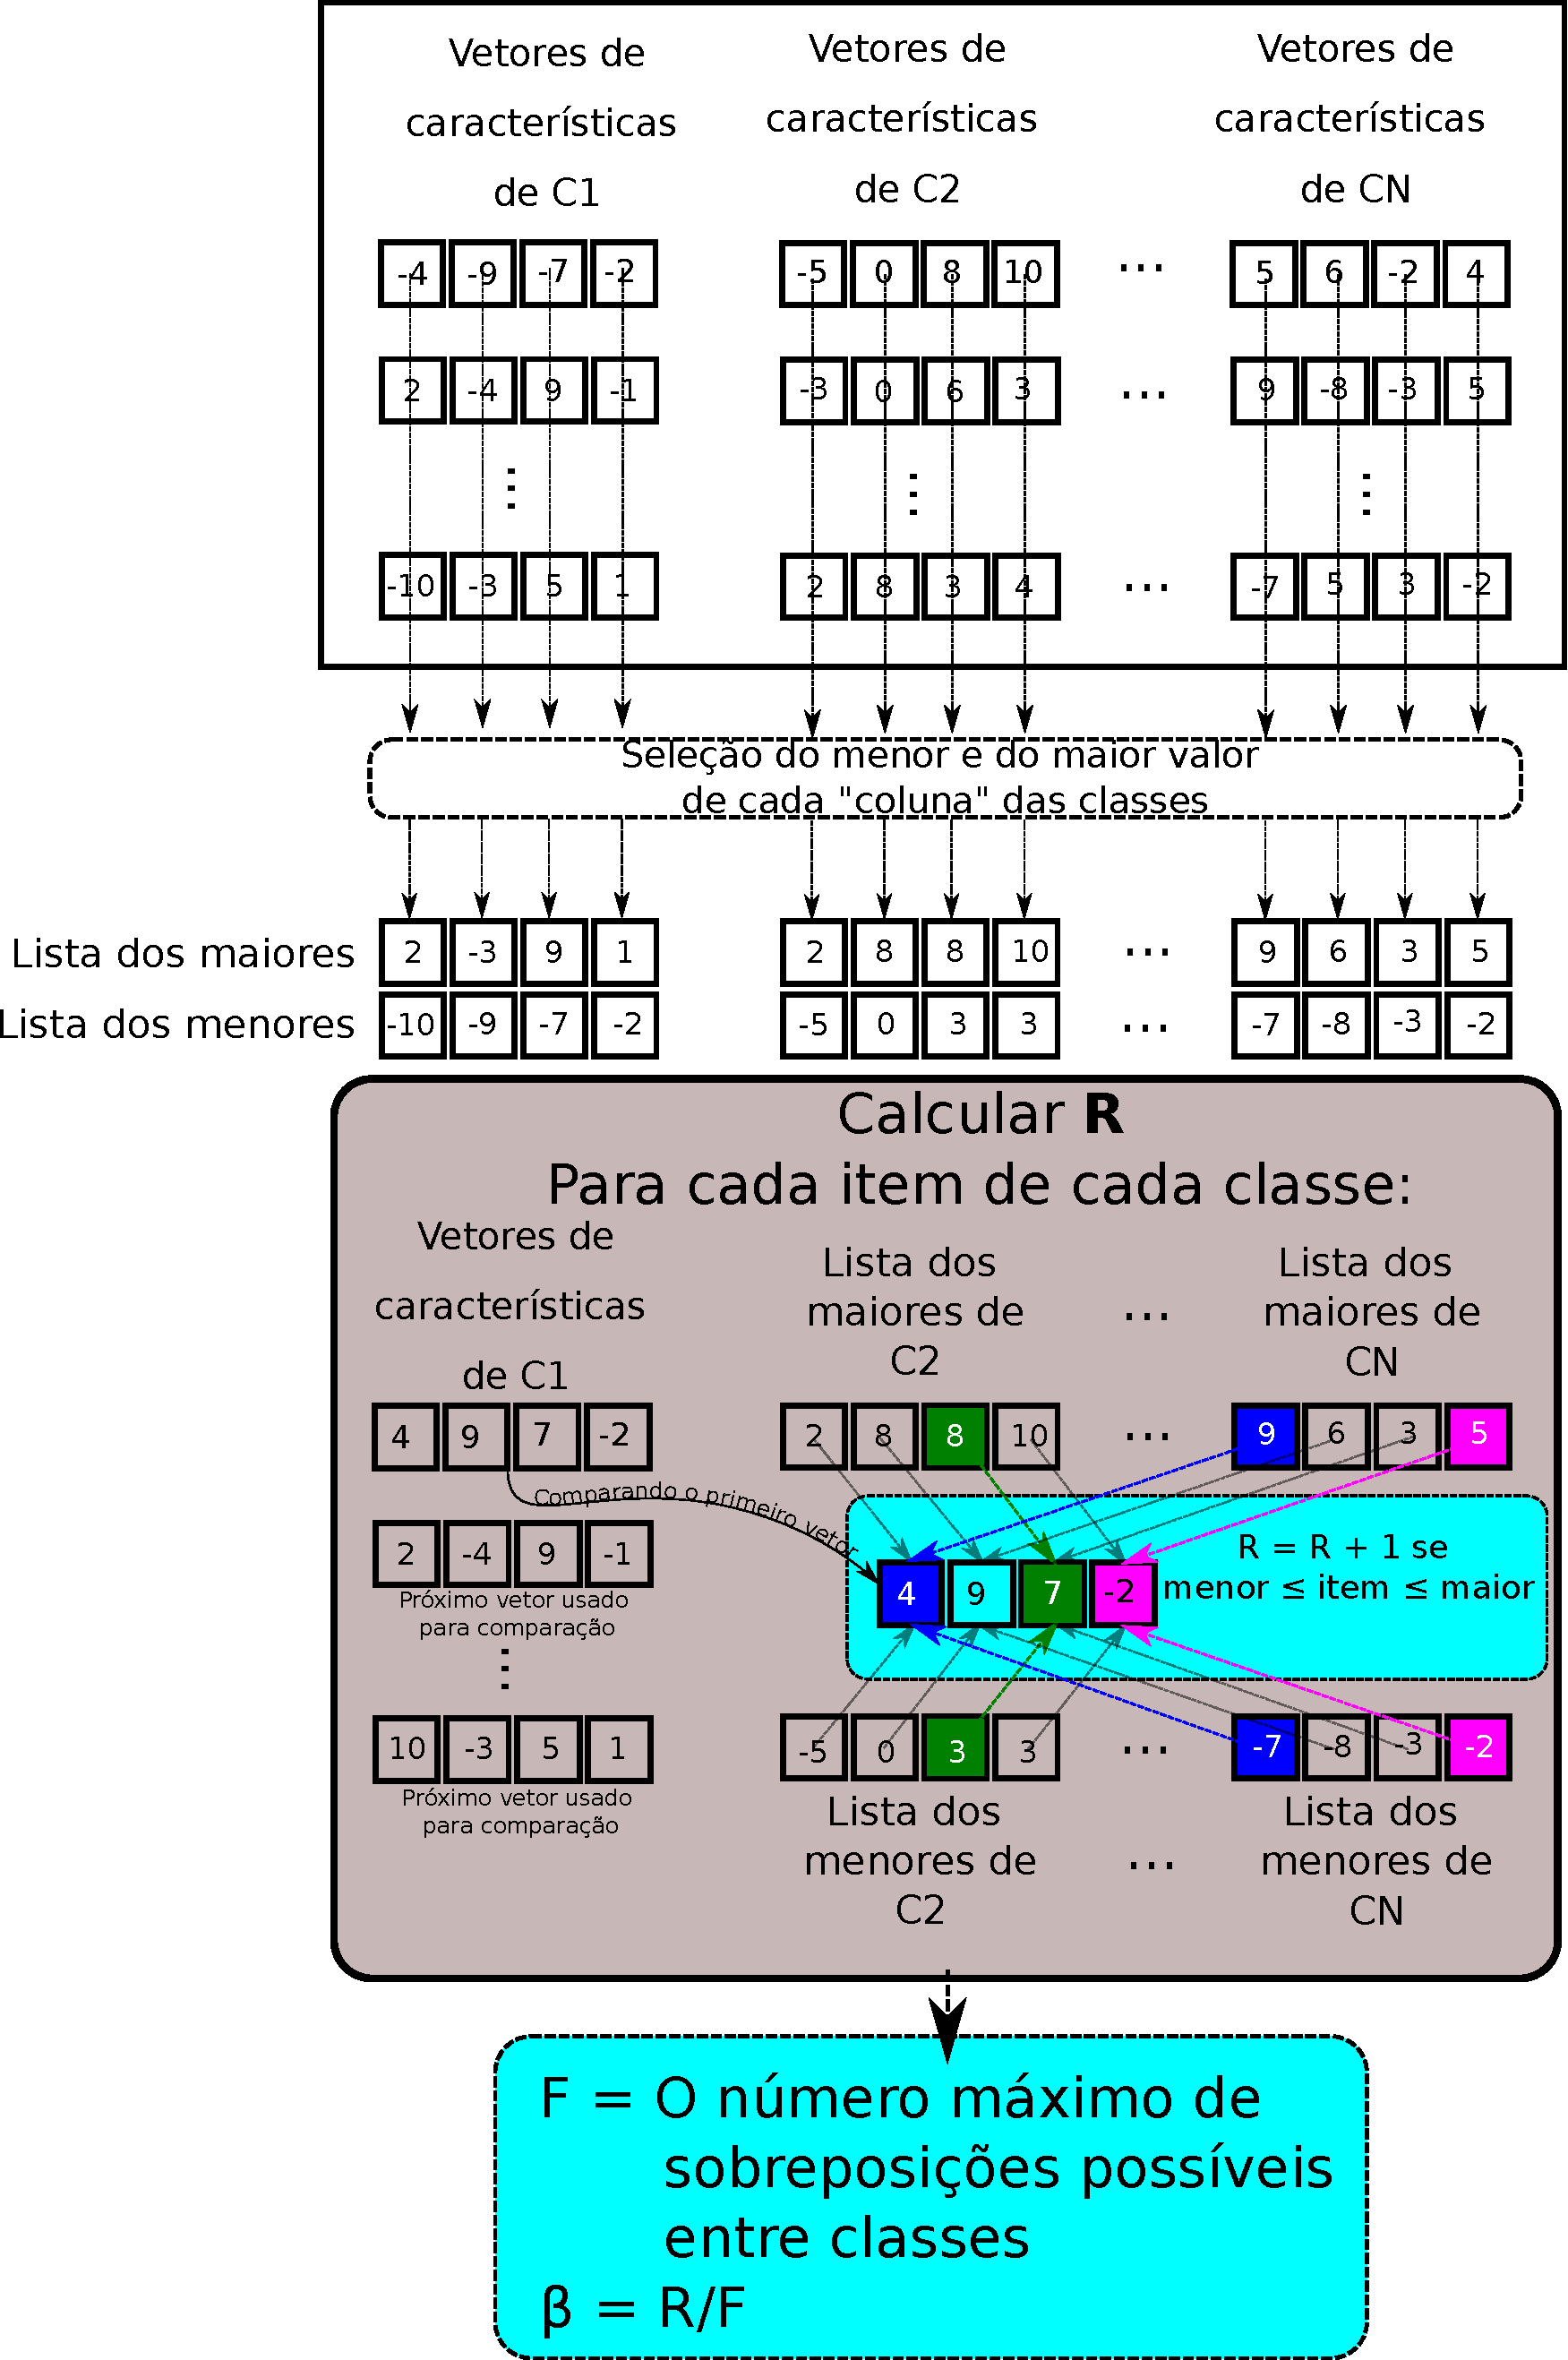
\includegraphics[height=.83\textheight]{../monography/images/betaCalculation.pdf}
			\end{textblock*}
			\column{.5\textwidth}
			\par Razão de sobreposição interclasse, $\beta$.
			\par $F = N.(N-1).X.T$
			\begin{itemize}
				\item N a quantidades de classes;
				\item X a quantidade de vetores de características por classe;
				\item T o tamanho do vetor de características.
			\end{itemize}
		\end{columns}
	}
	\only<3>{
		\framesubtitle{Graus de certeza e contradição}
		\begin{itemize}
			\item Grau de certeza $\rightarrow G_1=\alpha-\beta $.
			\item Grau de contradição $\rightarrow G_2=\alpha+\beta-1 $.				
		\end{itemize}
		Onde: $-1 \leqslant G_1 \leqslant 1$ e  $-1 \leqslant G_2 \leqslant 1\qquad$.\\
		Seja $P=(G_1,G_2)$
		\begin{itemize}
			\item \alert{Verdade $\rightarrow$ fé total ($\alpha = 1$) e nenhum descrédito ($\beta = 0$)}
			\item Ambiguidade $\rightarrow$ fé total ($\alpha = 1$) e descrédito total ($\beta = 1$)
			\item Falsidade $\rightarrow$ fé nula ($\alpha = 0$) e descrédito total ($\beta = 1$)
			\item Indefinição $\rightarrow$ fé nula ($\alpha = 0$) e nenhum descrédito ($\beta = 0$) \qquad.
		\end{itemize}
	}
	\only<4>{
		\framesubtitle{Distancias no plano paraconsistente}
		As distâncias$(D)$ do ponto $P=(G_1,G_2)$ dos limites supracitados. Tal cálculo pode ser feito da seguinte forma:
		\begin{equation*}
		D_{-1,0}=\sqrt{(G_1+1)^2+(G_2)^2}\qquad,
		\end{equation*}
		\alert{
			\begin{equation*}
			D_{1,0}=\sqrt{(G_1-1)^2+(G_2)^2}\qquad,
			\end{equation*}
		}
		\begin{equation*}
		D_{0,-1}=\sqrt{(G_1)^2+(G_2+1)^2}\qquad,		
		\end{equation*}
		\begin{equation*}
		D_{0,1}=\sqrt{(G_1)^2+(G_2-1)^2}\qquad,
		\end{equation*}
	}
	\only<5>{
		\framesubtitle{Os vetores de características proporcionam uma boa separação interclasses?\cite{8588433}}
		\begin{columns}
			\column{.5\textwidth}				
			\begin{figure}
				\centering
				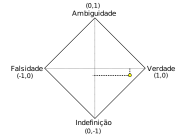
\includegraphics[width=.85\linewidth, angle=-90]{../monography/images/paraconsistentPlane}
				\label{fig:paraconsistentplane}
				\caption{Plano paraconsistente}
			\end{figure}
			\column{.5\textwidth}
			\begin{itemize}
				\item \alert{Verdade:\\
					$\alpha = 1$ e $\beta = 0$.}
				\item Ambiguidade:\\
				$\alpha = 1$ e $\beta = 1$.
				\item Falsidade:\\
				$\alpha = 0$ e $\beta = 1$.
				\item Indefinição:\\
				$\alpha = 0$ e $\beta = 0$.
			\end{itemize}
		\end{columns}
	}
\end{frame}
		\begin{frame}
	\frametitle{Autoencoders}
	\only<1>{
		\framesubtitle{Características de um autoencoder subcompleto}
		\begin{columns}
			\column{.3\linewidth}
				\par Exemplo esquemático de um \textit{autoencoder}: Os nós de entrada estão em cinza, a camada de código em amarelo contêm as características codificadas e finalmente a camada de reconstrução em vermelho contêm um cópia aproximada da entrada.
			\column{.7\linewidth}
				\begin{figure}[h]
					\centering
					\scalebox{.8}{
						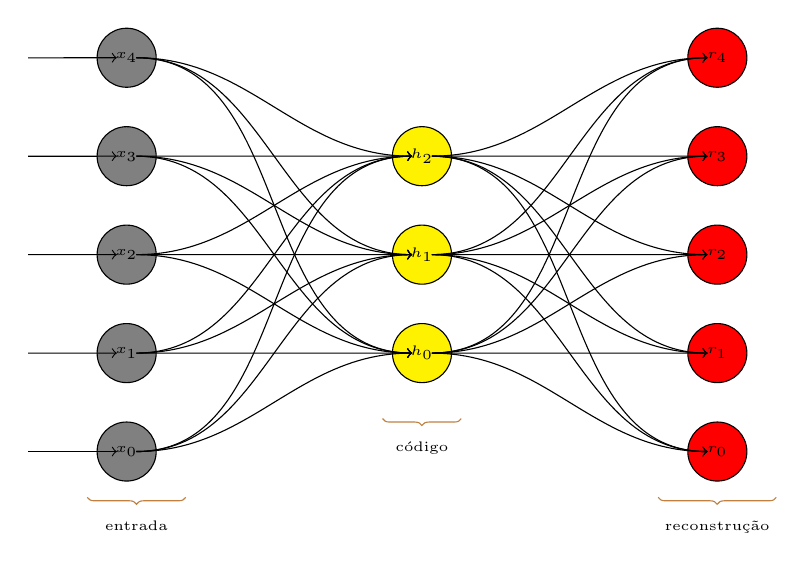
\begin{tikzpicture}[scale=2.5]
	% Define scaling factors
	\def\inputscale{.5}
	\def\hiddenscale{.5}
	\def\outputscale{.5}
	
	%input layer
	\foreach \i in {0,1,2,3,4} {
		\node (input_node\i) at (0,\i*\inputscale) {}; 
		\filldraw[fill=gray] (input_node\i) circle (0.15cm);
		\node at (input_node\i) {\tiny $x_\i$};
		
		\draw[->,in=180,out=0] (-0.5,\i*\inputscale) to (input_node\i);
	}
	
	%hidden layer
	\foreach \i in {0,1,2} {
		\node (hidden_node\i) at (1.5,\i*\hiddenscale+.5) {}; 
		\filldraw[fill=yellow] (hidden_node\i) circle (0.15cm);
		\node at (hidden_node\i) {\tiny $h_\i$};
	}
	
	%output layer
	\foreach \i in {0,1,2,3,4} {
		\node (output_node\i) at (3,\i*\outputscale) {}; 
		\filldraw[fill=red] (output_node\i) circle (0.15cm);
		\node at (output_node\i) {\tiny $r_\i$};
	}
	
	% Connect layers
	\foreach \i in {0,1,2,3,4} {
		\foreach \j in {0,1,2} {
			\draw[->,in=180,out=0] (input_node\i) to (hidden_node\j);
			\draw[->,in=180,out=0] (hidden_node\j) to (output_node\i);
		}
	}
	
	%descriptions
	\draw[snake=brace,mirror snake,raise snake=45pt,brown] (-0.2,0.4) -- (0.3,0.4) node[black,midway,yshift=-50pt,below]{\tiny entrada};
	
	\draw[snake=brace,mirror snake,raise snake=45pt,brown] (1.3,0.8) -- (1.7,0.8) node[black,midway,yshift=-50pt,below]{\tiny código};
	
	\draw[snake=brace,mirror snake,raise snake=45pt,brown] (2.7,0.4) -- (3.3,0.4) node[black,midway,yshift=-50pt,below]{\tiny reconstrução};

\end{tikzpicture}
					}
					\label{fig:autoencoder2}
				\end{figure}
		\end{columns}
	}
	\only<2>{
		\framesubtitle{Denoising}
		\par Representação funcional de um \textit{denoising autoencoder}: Sendo o vetor $x$ uma entrada e $n$ um função que adiciona um ruído aleatório então a informação com ruído $\hat{x}$ é definida como $\hat{x} = n(x)$, portanto o vetor $h$ é resultado da aplicação de uma função codificadora $f$ sobre $x$: $h = f(x)$, finalmente $r$ é a reconstrução de $x$ a partir $h$ através de uma função decodificadora $g$: $r = g(h)$. É importante notar que $r$ é comparada com $x$ e não com $\hat{x}$.
		
		\begin{figure}
			\centering
			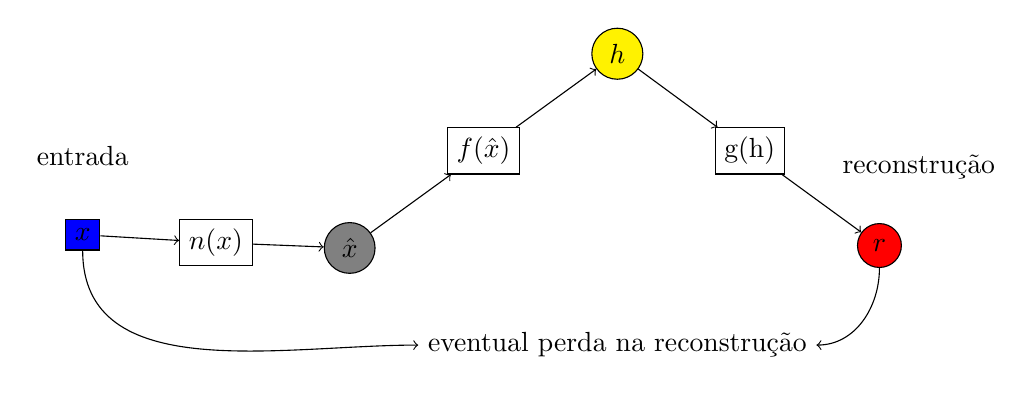
\begin{tikzpicture}[node distance=3cm, every edge/.style={draw=black,->}]
	% Nodes
	\node[draw, rectangle, fill=blue] (x) {$x$};
	
	\node[draw, rectangle, above right=-.6cm and 1cm of x] (noiser) {$n(x)$};
	
	\node[draw, circle, above right=-.6cm and 1cm of noiser, fill=gray] (x_hat) {$\hat{x}$};
	
	\node[draw, rectangle, above right=0.7cm and 1cm of x_hat] (encoder) {$f(\hat{x})$};
	
	\node[draw, circle, above right=0.7cm and 1cm of encoder, fill=yellow] (h) {$h$};
	
	\node[draw, rectangle, below right=0.7cm and 1cm of h] (decoder) {g(h)};
	
	\node[draw, circle, below right=0.7cm and 1cm of decoder, fill=red] (r) {$r$};
	
	% Arrows
	\draw (x) edge (noiser);
	\draw (noiser) edge (x_hat);
	\draw (x_hat) edge (encoder);
	\draw (encoder) edge (h);
	\draw (h) edge (decoder);
	\draw (decoder) edge (r);
	
	% Loss
	\node[below of=h, yshift=-0.7cm] (loss) {eventual perda na reconstrução};
	\draw [->,in=180,out=-90](x) edge (loss);
	\draw [->,in=0,out=-90] (r) edge (loss);
	
	% Labels
	\node[above of=x, yshift=-2cm] {entrada};
	\node[above of=r, yshift=-2cm, xshift=.5cm] {reconstrução};
\end{tikzpicture}
			\label{fig:denoisingAutoencoder}
		\end{figure}

	}
\end{frame}
		\begin{frame}
	\frametitle{Fala imaginada}
	\only<1>{
		\par A fala imaginada é um fenômeno em que uma pessoa "ouve" a si mesma falando internamente, sem produzir som. As regiões cerebrais usadas na fala imaginada são similares às que estão envolvidas na fala verbal, englobando áreas do córtex motor e pré-motor, além de outras áreas associadas à linguagem e a fala.
		
		\par A ativação cerebral durante processos linguísticos (incluindo a fala imaginada) envolve as seguintes regiões \cite{pinto2012manual}, \cite{Vanderah2020}, \cite{kenhub}:
		
		\begin{itemize}
			\item \textbf{área de Broca}: Produção da fala.
			\item \textbf{área de Wernicke}: Compreensão da linguagem.
			\item \textbf{córtex motor e pré-motor}: Articulação da fala.
			\item \textbf{giro supramarginal}: Planejamento motor da fala.
			\item \textbf{giro supratemporal e médio}: Compreensão linguística e articulação durante a repetição de sílabas.
		\end{itemize}
	}
	\only<2>{
		\framesubtitle{Visão geral do telencéfalo}
		\begin{figure}[p]
			\centering
			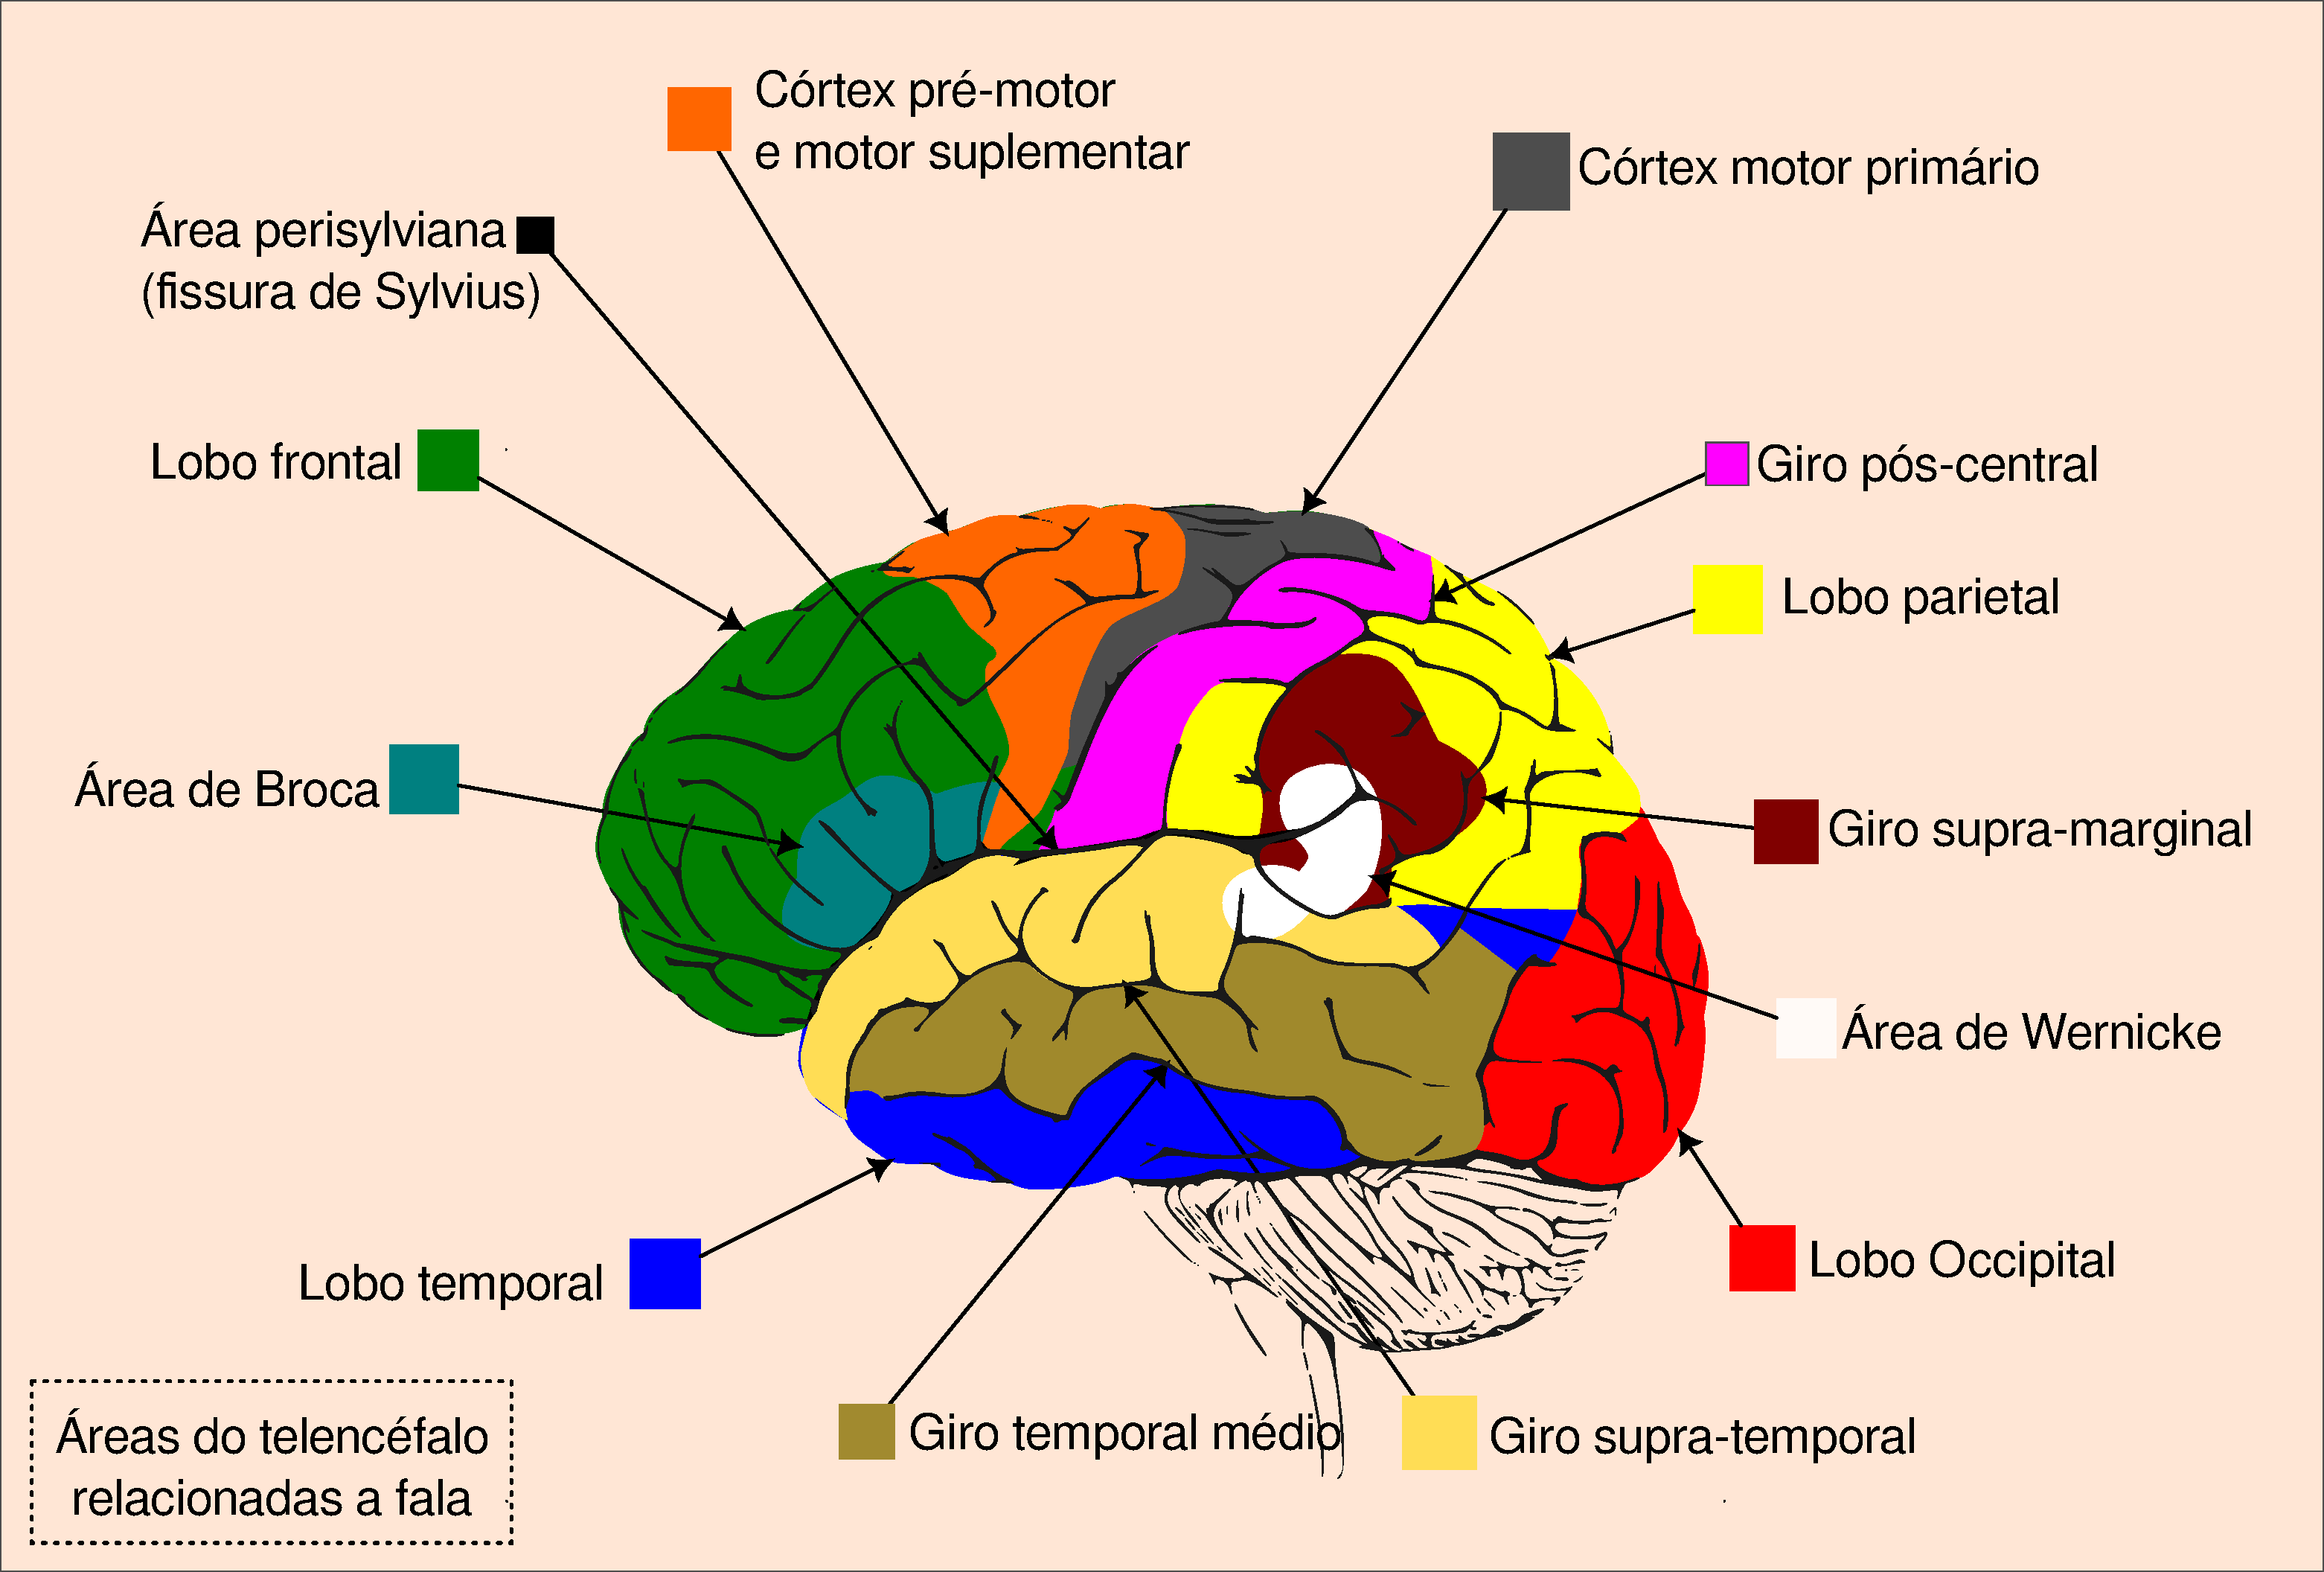
\includegraphics[width=.65\paperwidth,keepaspectratio]{../monography/images/teleencefaloTudo}
			\label{fig:teleencefalotudo}
		\end{figure}
	}
\end{frame}
		\begin{frame}
	\frametitle{Interfaces Humano-Máquina e EEG}
	
	\only<1>{
		\framesubtitle{EEG e as frequências do cérebro}
		\begin{columns}
			\column{.4\linewidth}
			\par \textbf{Eletroencefalograma}:
			\begin{itemize}
				\item não invasivo
				\item mais sujeito a ruídos
				\item exige tolerância a ruído
				\item mais econômico e simples de implementar
				\item eletrodos secos (reutilizáveis, mais interferência)
				\item eletrodos úmidos (não reutilizáveis, menos interferência)
			\end{itemize}
			\column{.6\linewidth}
			\begin{itemize}
				\item \textbf{Delta (1–4Hz)}: A onda mais lenta. Observada em bebês e durante o sono profundo em adultos.
				
				\item \textbf{Theta (4–8Hz)}: Observada em crianças, adultos sonolentos e durante a recordação de memórias.
				
				\item \textbf{Alpha (8–12Hz)}: Geralmente a banda de frequência dominante, aparecendo durante a consciência relaxada ou quando os olhos estão fechados.
				
				\item \textbf{Beta (12–25Hz)}: Associada ao pensamento, concentração ativa e atenção focada.
				
				\item \textbf{Gamma (acima de 25Hz)}: Observada durante o processamento sensorial múltiplo.
			\end{itemize}
		\end{columns}
	}
	
	\only<2>{
		\framesubtitle{Sistema 10-20}
		\begin{columns}
			\column{.4\linewidth}
				\par Posicionamento dos eletrodos de acordo com o padrão 10-20. Números ímpares são atribuídos aos eletrodos no hemisfério esquerdo, e números pares são atribuídos aos eletrodos no hemisfério direito \cite{sistema10-20}, \cite{JALALYBIDGOLY2020101788}.
			\column{.6\linewidth}
				\begin{figure}[h]
					\centering
					\includegraphics[width=1\linewidth]{../monography/images/10–20StandardAndLobes}
					\label{fig:1020standardandlobes}
				\end{figure}
		\end{columns}
	}
\end{frame}
		\begin{frame}
	\frametitle{Redes neurais de pulso (RNP)}
	
	
	\only<1>{
		\framesubtitle{Características}
		\begin{itemize}
			\item funciona segundo limiares de ativação.
			\item redes esparsas (baixa ativação sináptica).
			\item uso de pulsos em vez de valores contínuos.
			\item processamento orientado ao tempo \cite{10242251}.
			\item tolerantes a ruídos (atuam como um filtro passa baixa).
			\item não um simulação de um-para-um como o neurônio Hodgkin-Huxley. \cite{gerstner2014neuronal} ou outros \cite{jones2020single}.
		\end{itemize}
	}
	
	\only<2>{
		\framesubtitle{\textit{Leaky Integrate and Fire Neurons} (LIF)}
		\begin{columns}
			\column{.5\linewidth}
				\begin{itemize}
					\item se assemelha com circuitos Resistor-Capacitor.
					\item os pulsos são representados como \textbf{uns} dispersamente distribuídos em uma sequência de \textbf{zeros}
					\item simples, mais eficientes e atualmente generalizam melhor para a maioria dos problemas \cite{dan_goodman_2022_7044500}.
				\end{itemize}
			\column{.5\linewidth}
			
			\begin{figure}[h]
				\centering
				\caption[Modelo RC]{O modelo RC}
				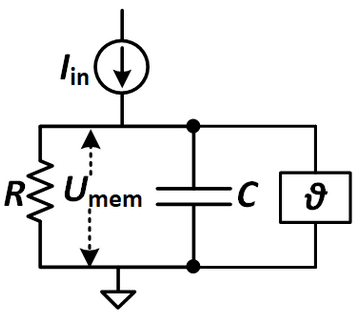
\includegraphics[width=.5\linewidth]{../monography/images/rcmodel}
				\label{fig:rcmodel}
			\end{figure}
		\end{columns}
	}
	\only<3>{
		\framesubtitle{\textit{Leaky Integrate and Fire Neurons} (LIF)}
		\par Gráfico do LIF simulado completo.
		\begin{figure}[H]
			\centering
			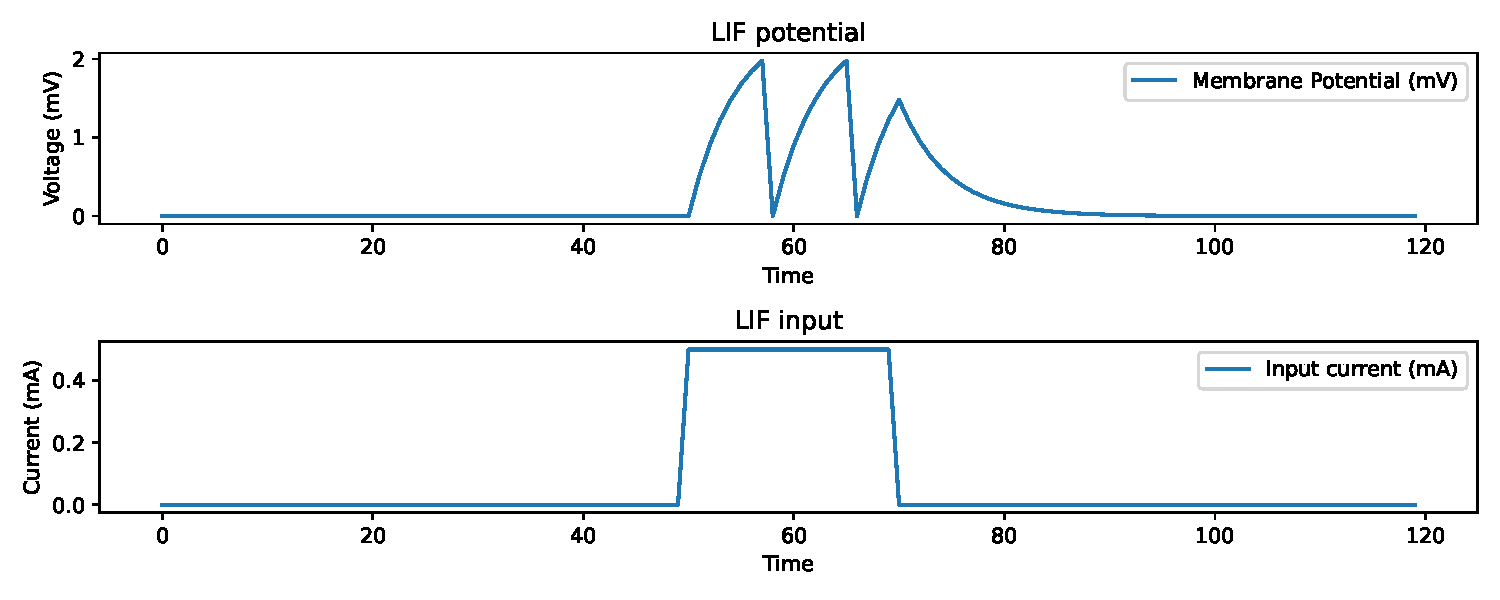
\includegraphics[width=.8\linewidth]{../monography/images/membranePotentialFull}
			\label{fig:membranepotentialfull}
		\end{figure}
	}
	\only<4>{
		\framesubtitle{Esparsidade}
		\par Atividade dispersa de uma RNP: O eixo horizontal representa o momento no qual os dados estão sendo processados e o vertical representa o número do neurônio (índice) na RNP. Note que, na maior parte do tempo, muito poucos neurônios são ativados.
		\begin{figure}[h]
			\centering
			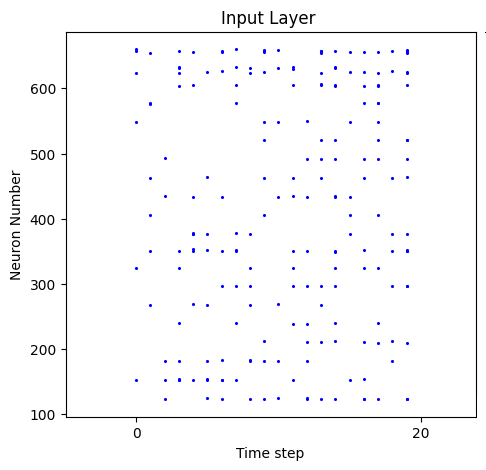
\includegraphics[width=.4\linewidth]{../monography/images/sparsity}
			\label{fig:sparsity}
		\end{figure}
	}
	
	\only<5>{
		\framesubtitle{Treinamento}
		\begin{itemize}
			\item \textbf{Plasticidade Dependente do Tempo de Pulsos (STDP)}: Se um neurônio pré-sináptico dispara \textbf{antes} do pós-sináptico, há um fortalecimento na conexão, mas se o neurônio pós-sináptico disparar antes, então há um enfraquecimento.
			\item \textbf{Descida de Gradiente Emprestada}: Aproxima a função de passo usando outra função matemática, que é diferenciável (como uma sigmoide), para treinar a rede. Essas aproximações são usadas apenas na fase de \textit{backpropagation}, enquanto mantêm a função de passo na fase do \textit{feed-forward}.
			\item \textbf{Algoritmos Evolutivos}: Usam a seleção dos mais aptos ao longo de muitas gerações de redes.
			\item \textbf{Reservatório/Computação Dinâmica}: \textbf{Redes de estado de eco} ou \textbf{Máquinas de estado líquido}, respectivamente.
		\end{itemize}
	}	
\end{frame}
		\begin{frame}
	\frametitle{Redes neurais residuais (ResNets)}
	
	\only<1>{
		\par Redes neurais profundas podem sofrer com desaparecimento ou explosão do gradiente. A solução é reproduzir o comportamento de redes neurais mais rasas usando conexões de salto. Essa é ideia das redes neurais residuais.
	}
	
	\only<2>{
		\begin{columns}
			\column{.5\linewidth}
				\begin{figure}[H]
					\centering
					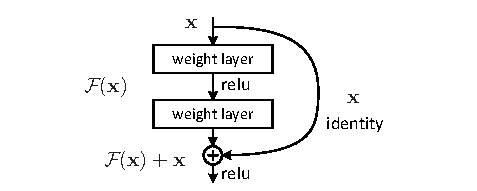
\includegraphics[width=1\linewidth]{../monography/images/residualBlock}
					\label{fig:residualblock}
				\end{figure}
			\column{.5\linewidth}
				\par Segundo \cite{DBLP:journals/corr/HeZRS15} a ideia-chave por trás das \textit{ResNets} é a inclusão de conexões de salto como ilustrado na  figura ao lado, também conhecidas como mapeamentos de identidade.
				
				\par Bloco Residual: $x$ contorna as camada intermediárias $F(x)$ via uma função identidade somando-se a $F(x)$ ao final do bloco.
		\end{columns}
	}
	
	\only<3>{
		\par Obtenção do resíduo: $x$ um vetor de entrada na rede, $I(\cdot)$ é uma função identidade cujo valor é diretamente somado $\oplus$ com o resultado produzido pelas várias camadas representadas por $f(\cdot)$, $h$ é um vetor representando um estado intermediário de uma rede neural.
		\begin{figure}[h]
			\centering
			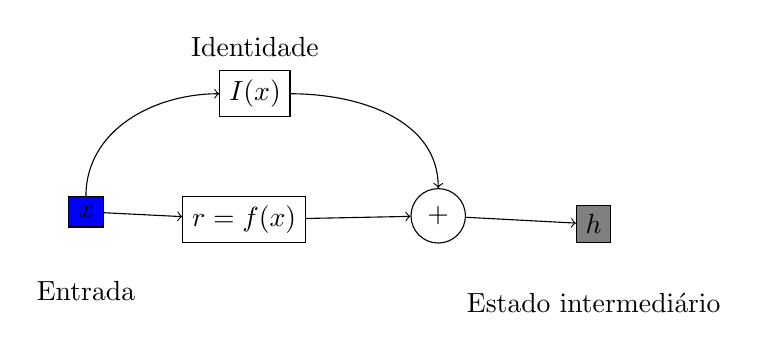
\begin{tikzpicture}[node distance=3cm, every edge/.style={draw=black,->}]
	% Nodes
	\node[draw, rectangle, fill=blue] (x) {$x$};
	\node[draw, rectangle, above right=-.6cm and 1cm of x] (function) {$r = f(x)$};
	\node[draw, rectangle, above right=1cm and -1.1cm of function] (identi) {$I(x)$};
	\node[draw, circle, above right=-.5cm and 4cm of x] (plus) {$+$};
	\node[draw, rectangle, above right=-.6cm and 1.5cm of plus, fill=gray] (hidden) {$h$};
	
	% Arrows
	\draw (x) edge (function);
	\draw (function) edge (plus);
	\draw (plus) edge (hidden);
	
	
	\draw [->,in=180,out=90](x) edge (identi);
	\draw [->,in=90,out=0] (identi) edge (plus);
	

	% Labels
	\node[above of=identi, yshift=-2.4cm] {Identidade};
	\node[above of=x, yshift=-4cm] {Entrada};
	\node[above of=hidden, yshift=-4cm, xshift=0cm] {Estado intermediário};
\end{tikzpicture}
			\label{fig:residuo}
		\end{figure}
	}
\end{frame}
	
	\section{Estado-da-arte em autenticação por voz e fala imaginada}
		\begin{frame}[allowframebreaks]
	\frametitle{Trabalhos}
	\begin{itemize}
		
		\item \textbf{Classificação e tratamento de EEG:} \begin{itemize}
			\item O estudo de \cite{ParkHyeong-jun2023Mcoi} explora o uso de EEG para fala imaginada com NA-MEMD e DTWPT, usando MRF-CNN para classificar sinais decompostos. A acurácia média foi 80,41\%.
			
			\item Em \cite{AbdulghaniMokhlesM2023ISCU}, utilizou-se Wavelet Scattering Transform (WST) e uma Rede Neural LSTM para classificar expressões imaginadas, alcançando 92,50\% de acurácia.
			
			\item O estudo \cite{MahapatraNrushinghCharan2023Ecoi} usou DTWT para processar sinais EEG e alcançou acurácias de 98,18\% e 71,60\% nas bases MUSE e EPOC, respectivamente.
			
			\item A revisão em \cite{ShahUzair2022TRoA} destacou o uso de filtros Wavelet e algoritmos SVM e CNN, sugerindo a inclusão de métricas como Precisão e Recall para uma visão mais completa.
			
			\item O estudo \cite{MahapatraNrushinghCharan2022MCoI} aplicou uma combinação de TCN e CNN com FastICA e DTWT para sinais EEG, alcançando 96,49\% de acurácia.
			
			\item \cite{AgarwalPrabhakar2022Ebia} usou DTWT e dois algoritmos (RF e SVM) para classificar letras imaginadas, obtendo 77,97\% de acurácia. Utilizou também CAR para melhorar a SNR.
			
			\item O trabalho em \cite{Hernandez-Del-ToroTonatiuh2021TaEB} usou DTWT, EMD e características baseadas em teoria do caos, alcançando melhores resultados com RF, KNN, SVM e Regressão Logística.
			
			\item Em \cite{MOCTEZUMA2019201}, CAR foi combinado com DTWT e TEO para melhorar a SNR, alcançando uma acurácia de 97\% com 5 voluntários.
			
			\item \cite{PanachakelJerrinRamakrishnan} usou janelas deslizantes e matrizes tridimensionais para classificar sinais EEG, alcançando acurácias de 79,7\% a 95,5\%.
			
			\item \cite{tamm2020classification} simplificou uma CNN com transferência de aprendizado, alcançando uma acurácia de 23,98\% em uma base de dados reduzida.
			
			\item O estudo de \cite{Panachakel_2019} aplicou transformadas Wavelet de nível 7 e obteve 57,15\% de acurácia ao tratar separadamente os vetores de características.
			
			\item \cite{panachakel2020novel} usou uma rede neural profunda e transformada wavelet para duas palavras, alcançando 71,8\% de acurácia.
			
			\item A revisão em \cite{s23125575} mostrou que SVM, RF, HMM e GMM foram comuns, com técnicas profundas como CNN e RNN emergindo desde 2020.
		\end{itemize}
		
		
		%%%%%
		
		\item \textbf{Classificação e tratamento de voz:} \begin{itemize}
			
			\item \cite{math11194205} combinou Res2Net com PWPE e ECA, alcançando menos de 8\% de EER em contextos variados.
			
			\item O estudo de \cite{ali2022speech} focou na classificação do gênero usando MFCC e LPC, alcançando 97,07\% de acurácia com redes neurais artificiais.
			
			\item \cite{WOS:000525844000004} introduziu o sistema AVA para autenticação ativa, com uma taxa média de WEER de 3\% a 4\%.
			
			\item O estudo \cite{10.1145/3448113} explorou microfones em fones para criar impressões digitais auditivas, alcançando um EER de 3,64\%.
			
			\item \cite{9744556} usou sons de estalos para prevenção de spoofing, alcançando uma classificação baseada em vetores de características de 3 dimensões.
			
			\item O estudo \cite{furlan2021caracterizacao} comparou métodos baseados em distâncias e SVM, alcançando mais de 99\% de precisão usando a escala BARK e wavelet Haar.

		\end{itemize}
	\end{itemize}
\end{frame}
\begin{frame}
	\frametitle{Trabalhos - Conclusões}
	\par Os estudos analisados contribuíram para a construção do protocolo de coleta de dados, abordando a importância de filtrar interferências da rede elétrica local e a separabilidade dos canais EEG usando o algoritmo \textit{FastICA}. A fase de extração de características é crucial para o desempenho dos algoritmos de classificação. Também é importante a separação dos indivíduos por sexo, destros e canhotos, além da consideração das ondas cerebrais $\alpha$, $\beta$ e $\theta$ isoladamente ou em conjunto. Técnicas como DTWT e CAR são comuns na literatura. Estudos demonstram que redes neurais profundas não necessariamente superam redes rasas, e o uso de sinais EEG separados por canal para aumentar a quantidade de dados é uma abordagem interessante. Além disso, técnicas para extração de características continuam como um das partes mais importantes no projeto de sistemas de análise e reconhecimento de sinais.
	
\end{frame}
\begin{frame}[allowframebreaks]
	\frametitle{Comparativo - Referências}
	
	\par \textbf{Escalas de energia usadas}
	\begin{itemize}
		\item Energia de Teager (TEO): Usada para extração de características em \cite{MOCTEZUMA2019201}.
		\item Energia de bandas: Obtida usando DTWT para cada banda de frequência em \cite{Hernandez-Del-ToroTonatiuh2021TaEB}.
	\end{itemize}
	
	\par \textbf{Tipos de classificadores usados}
	\begin{itemize}
		\item Redes Neurais Convolucionais (CNN): Usadas em \cite{PanachakelJerrinRamakrishnan}, \cite{MahapatraNrushinghCharan2022MCoI}.
		\item Redes Neurais Recorrentes LSTM (Long-Short Term Memory): Usadas em \cite{AbdulghaniMokhlesM2023ISCU}.
		\item Support Vector Machines (SVM): Usadas em \cite{ShahUzair2022TRoA}, \cite{Hernandez-Del-ToroTonatiuh2021TaEB}.
		\item Random Forest (RF): Usado em \cite{AgarwalPrabhakar2022Ebia}, \cite{Hernandez-Del-ToroTonatiuh2021TaEB}, \cite{MOCTEZUMA2019201}.
		\item Bidirectional Recurrent Neural Networks: Usadas em \cite{MahapatraNrushinghCharan2023Ecoi}.
		\item Deep Neural Networks (DNN): Usadas em \cite{Panachakel_2019}, \cite{panachakel2020novel}.
		\item Hidden Markov Model (HMM): Usado em \cite{WOS:000525844000004}.
		\item Análise Discriminante e redes neurais artificiais: Usadas em \cite{ali2022speech}.
		\item ResNet50 com transferência de aprendizado: Usado em \cite{PanachakelJerrinRamakrishnan}.
	\end{itemize}
	
	\par \textbf{Técnicas de extração de características}
	\begin{itemize}
		\item Transformada Wavelet Discreta (DTWT): Usada em \cite{MahapatraNrushinghCharan2023Ecoi}, \cite{Hernandez-Del-ToroTonatiuh2021TaEB}.
		\item Empirical Mode Decomposition (EMD): Usada em \cite{ParkHyeong-jun2023Mcoi}.
		\item Wavelet Scattering Transform (WST): Usada em \cite{AbdulghaniMokhlesM2023ISCU} e \cite{Panachakel_2019}.
		\item FastICA (Independent Component Analysis): Usada em \cite{MahapatraNrushinghCharan2022MCoI}.
		\item Mel-Frequency Cepstral Coefficients (MFCC): Usada em \cite{ali2022speech}, \cite{WOS:000525844000004}.
		\item Linear Prediction Coefficients (LPC): Usados em \cite{ali2022speech}.
		\item Teager Energy Operator (TEO): Usado em \cite{MOCTEZUMA2019201}.
		\item Fourier Transform: Usada para alguns dados em \cite{s23125575}.
		\item Common Average Referencing (CAR): Usado em \cite{AgarwalPrabhakar2022Ebia}, \cite{Hernandez-Del-ToroTonatiuh2021TaEB}, \cite{MOCTEZUMA2019201}.
		\item Dimensionamento fractal e métodos da teoria do Caos: Usados em \cite{Hernandez-Del-ToroTonatiuh2021TaEB}.
	\end{itemize}
\end{frame}
\begin{frame}
	\frametitle{Comparativo - Tese}
		\par \textbf{Escalas de energia usadas}
		\begin{itemize}
			\item energia das bandas na escala BARK
			\item energia das bandas na escala MEL
			\item energia das bandas $\alpha$, $\beta$, $\gamma$, $\theta$ e $\delta$
		\end{itemize}
		
		\par \textbf{Tipos de classificadores usados}
		\begin{itemize}
			\item Redes neurais de pulso (SNN)
			\item Redes neurais residuais (RNN)
		\end{itemize}
		
		\par \textbf{Técnicas de extração de características}
		\begin{itemize}
			\item Transformada Wavelet Discreta (DTWT)
			\item Mel-Frequency Cepstral Coefficients (MFCC)
			\item Auto-encoders
		\end{itemize}
\end{frame}

	\section{Abordagem proposta}
		\begin{frame}
	\frametitle{A Base de Sinais de Voz}
	\only<1>{
		\framesubtitle{Coleta dos dados}
		\begin{itemize}
			\item 20 pessoas.
			\item Ambos sexos.
			\item Idades entre 7 e 67 anos.
			\item Dígitos falados de 0 a 9.
			\item Língua portuguesa e inglesa.
			\item Total de 820 sinais entre genuínos e falsificados.
			\item Quantização de 16 bits.
			\item Taxa de amostragem 44100Hz.
		\end{itemize}
	}
	\only<2>{
		\framesubtitle{Organização dos dados}
		\begin{textblock*}{\linewidth}(0cm,0.4cm)
			\begin{figure}[t]
				\centering
				\subfloat[0.33\textwidth][Base em nível 1]{
					\includegraphics{../monography/images/directoryStructLevel01.pdf}
					\label{fig:directorystructlevel01}
				}
				\subfloat[0.33\textwidth][Base em nível 2]{
					\includegraphics{../monography/images/directoryStructLevel02.pdf}
					\label{fig:directorystructlevel02}
				}
				\subfloat[0.33\textwidth][Base em nível 3]{
					\includegraphics{../monography/images/directoryStructLevel03.pdf}
					\label{fig:directorystructlevel03}
				}
				\caption{Organização da base de dados}
				\label{fig:directorystructlevel010203}
			\end{figure}
		\end{textblock*}
	}
\end{frame}
		\begin{frame}
	\frametitle{Estrutura da Estratégia Proposta}
		\only<1>{
			\framesubtitle{Diagrama}
			\begin{textblock*}{\linewidth}(0.3cm,2cm)
				\begin{figure}[h]
					\centering
					\scalebox{0.75}	{
						\begin{figure}[h]
	\centering
	\caption{Estrutura da estratégia proposta}
	\scalebox{0.75}	{
		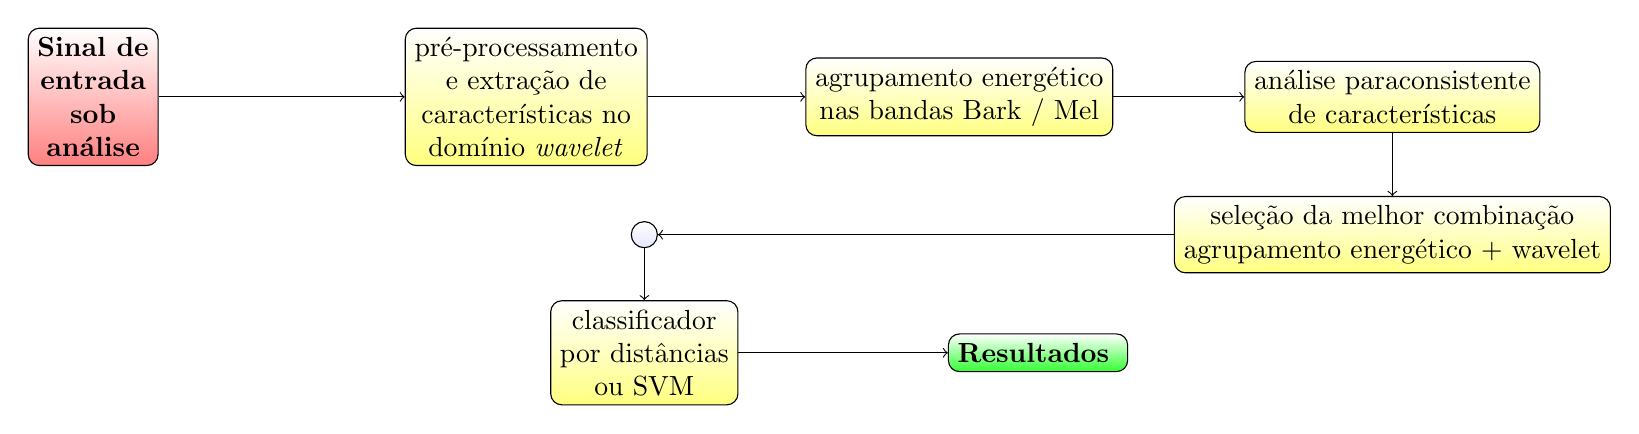
\begin{tikzpicture} 
			\node (z1)[shape=rectangle, rounded corners, draw, align=center, top color=white, bottom color=red!50] 
			at (0,2){
				\textbf{Sinal de} \\ \textbf{entrada} \\ \textbf{sob} \\ \textbf{análise}
			}; 
				
			\node (z2)[shape=rectangle, rounded corners, draw, align=center, top color=white, bottom color=yellow!50] 
			at (5.5,2){
				pré-processamento \\ e extração de \\ características no \\ domínio \textit{wavelet}
			}; 	
			
			\node (z3)[shape=rectangle, rounded corners, draw, align=center, top color=white, bottom color=yellow!50] 
			at (11,2){
				agrupamento energético \\ nas bandas Bark / Mel
			}; 	
			
			\node (z4)[shape=rectangle, rounded corners, draw, align=center, top color=white, bottom color=yellow!50] 
			at (16.5,2){
				análise paraconsistente \\ de características
			}; 
			
			\node (z5)[shape=rectangle, rounded corners, draw, align=center, top color=white, bottom color=yellow!50] 
			at (16.5,0.25){
				seleção da melhor combinação \\ agrupamento energético + wavelet
			}; 
					
			\node (z6)[shape=circle, draw, align=center, top color=white, bottom color=blue!10] 
			at (7,0.25) {};
			
			\node (z7)[shape=rectangle, rounded corners, draw, align=center, top color=white, bottom color=yellow!50] 
			at (7,-1.25) {
				classificador \\ por distâncias \\ ou SVM
			};
			
			\node (z8)[shape=rectangle, rounded corners, draw, align=center, top color=white, bottom color=green!80] 
			at (12,-1.25) {
				\textbf{Resultados}
			};
			
			\path[->] (z1) edge (z2);
			\path[->] (z2) edge (z3);
			\path[->] (z3) edge (z4);
			\path[->] (z4) edge (z5);
			\path[->] (z5) edge (z6);
			\path[->] (z6) edge (z7);	
			\path[->] (z7) edge (z8);
		\end{tikzpicture}
	}
	\label{fig_arq}
	\\Fonte: Elaborado pelo autor, 2021.
\end{figure}
					}
				\end{figure}
			\end{textblock*}
		}
		\only<2>{
			\framesubtitle{Wavelets inicialmente usadas}
				\begin{itemize}
					\item Haar.
					\item Beylkin com suporte 18.
					\item Vaidyanathan de suporte 24.
					\item Daubechies de	suportes 4 até 76.
					\item Symmlets com suportes 8, 16 e 32.
					\item Coiflets com suportes 6, 12, 18, 24 e 30.
				\end{itemize}
		}
		\only<3>{
			\framesubtitle{Métricas}
				\begin{itemize}
					\item Tabela de confusão.
					\begin{itemize}
						\item EER (Equal Error Rate).
						\item Acurácia e seu respectivo desvio padrão.
					\end{itemize}
					\item pontuação F1
					\item precisão
					\item recall
					\item Erro Médio Quadrático
					\item área sob a Curva ROC
					\item sensitividade
					\item especificidade
				\end{itemize}
		}
%		\only<4>{
%			\framesubtitle{Acurácia e EER}
%				\begin{columns}
%					\column{.5\textwidth}
%					\begin{equation}
%						acuracia = \dfrac{TP + TN}{N} \qquad,
%						\label{eq:calculoDaAcuracia}
%					\end{equation}
%					
%					\column{.5\textwidth}
%					\par São calculadas tabelas de confusão por um número suficiente de vezes até que \textbf{\textit{FAR} = \textit{FRR} = \textit{EER}}, a cada ciclo os vetores de características são comutados de forma aleatória.\newline
%
%					\begin{equation}
%						FAR=\dfrac{FP}{TN+FP} \qquad,
%						\label{eq:FAR}
%					\end{equation}
%					
%					\begin{equation}
%						FRR=\dfrac{FN}{TP+FN} \qquad,
%						\label{eq:FRR}
%					\end{equation}
%				\end{columns}
%		}
\end{frame}
	
	\begin{frame}[allowframebreaks]
		\frametitle{Referências}
		\bibliography{../monography/bibliography.bib}
	\end{frame}
	
\end{document}